\documentclass[runningheads]{llncs}

\usepackage{graphicx}
\usepackage{hyperref}
\usepackage{multicol}
\usepackage{listings}
\usepackage{natbib}

%%%%%%%%%%%%%%%%%%%%%%%%%%%%%%%%%%%%%%%%%%%%%%%%%%%%%%

\begin{document}
\title{Inequality of opportunity in the research career: a quantitative analysis.}
\author{Alberto Morales Galán
\and
Oriol Colomé Font}
%%%%%%%%%%%%%%%%%%%%%%%%%%%%%%%%%%%%%%%%%%%%%%%%%%%%%%
\institute{Universitat Pompeu Fabra, Barcelona \and
\email{\{alberto.morales01, oriol.colome01\}@estudiant.upf.edu}\\
\url{http://www.upf.edu}}
%%%%%%%%%%%%%%%%%%%%%%%%%%%%%%%%%%%%%%%%%%%%%%%%%%%%%%
\maketitle              % typeset the header of the contribution
%%%%%%%%%%%%%%%%%%%%%%%%%%%%%%%%%%%%%%%%%%%%%%%%%%%%%%
\begin{abstract}
This meta-research analysis shines a spotlight on the inequality of opportunity in research careers and seeks to identify the areas receiving the most academic attention. In a world where social movements have underscored the need for increased diversity, equity, and inclusion, it is crucial to examine the existing literature on discrimination in academia. We focus on the most extensively researched factors of discrimination to discern where the majority of investigative efforts are channeled.

Employing the SCOPUS database, we selected and analyzed a set of articles that addressed discrimination in academia. Our results highlight the preponderance of gender discrimination studies, reflecting over 75\% of the analyzed articles. However, we also noticed an increasing trend in studies on racial discrimination and other less-researched areas such as sexual orientation discrimination, ageism, and ableism.

Our study underscores the importance of broadening the scope of academic investigation to other underrepresented areas of discrimination. Further, it advocates for the persistent push towards equality of opportunity in research careers.

\keywords{Discrimination \and Inequality \and Equality \and Discrimination in Science \and Inequality in Science \and Research Career \and Meta-Research Analysis}
\end{abstract}

%%%%%%%%%%%%%%%%%%%%%%%%%%%%%%%%%%%%%%%%%%%%%%%%%%%%%%
%%%%%%%%%%%%%%%%%%%%%%%%%%%%%%%%%%%%%%%%%%%%%%%%%%%%%%
%%%%%%%%%%%%%%%%%%%%%%%%%%%%%%%%%%%%%%%%%%%%%%%%%%%%%%
\section{Introduction}
The recent upsurge of social protest movements such as \#MeToo \cite{joanpere2022history} and \#BlackLivesMatter \cite{nguyen2022black} have drawn global attention to the pressing issues of diversity, equity, and inclusion. These calls for systemic change resonate in all corners of society, including scientific institutions worldwide. Yet, while these institutions are critical drivers of innovation and progress, there are growing concerns that not all members of society have equal opportunities to participate and succeed in these settings. This systematic discrimination, defined as the unjust or prejudicial treatment of different categories of people, is an issue that merits rigorous scientific investigation.

Given the significance of this issue, we have embarked on a meta-research analysis to understand better the dynamics of inequality of opportunity in scientific research careers. Our aim is to uncover the current state of affairs and reveal how the academic discourse on this topic has evolved over the past five years. This study's findings may be useful in informing policy interventions and stimulating further research.

The significance of our research lies in its potential to provide a systematic review of the current state of the academic literature concerning inequality and discrimination in academic and research careers. It is well-documented that various forms of discrimination persist in academia and research fields, often hindering the progress and careers of marginalized groups \cite{shor2015paper}.

\subsection{Research question(s)}
Guiding our study are the following research questions:
\begin{itemize}
\item Are there instances of discrimination when accessing a research career?
\item What are the potential causes or sources of this discrimination?
\item What trends or patterns have emerged over the past five years in the study of this phenomenon?
\end{itemize}

The answers to these questions could shed light on the underpinnings of discrimination in research careers and help identify possible countermeasures.

%%%%%%%%%%%%%%%%%%%%%%%%%%%%%%%%%%%%%%%%%%%%%%%%%%%%%%

\section{Methodology}
Our meta-research analysis employed the \href{https://www.scopus.com/}{SCOPUS} database, an extensive multidisciplinary database comprising scientific publications from various disciplines. SCOPUS's unique combination of an expertly curated abstract and citation database, enriched data, and linked scholarly literature facilitates finding relevant and authoritative research, identifying experts, and providing access to reliable data, metrics, and analytical tools.

\subsection{Research Procedure}
Our analysis involved the selection and analysis of articles that met specific criteria. We focused on articles that addressed the issue of discrimination in academia, irrespective of the underlying cause. This approach allowed us to create a comprehensive dataset that we could then scrutinize to identify patterns or trends concerning the types of discrimination reported in the literature. 

Importantly, we defined our dataset beforehand to avoid introducing bias into our analysis.

\subsection{Criteria for Inclusion and Analysis}
Our focus primarily centered on understanding how these constructs intersect with academic and research careers. To establish our dataset, we employed specific criteria: articles were included if their titles or abstracts contained any of the terms: "\textbf{\textit{inequality}}", "\textbf{\textit{discrimination}}", "\textbf{\textit{equality}}", "\textbf{academic career}", or "\textbf{\textit{research career}}". This allowed us to create a comprehensive dataset that could adequately represent the breadth of existing literature on these issues.

\subsubsection{SCOPUS QUERY}
The following SCOPUS query was used to identify relevant articles:

\textit{(TITLE-ABS-KEY (inequality) OR TITLE-ABS-KEY (equality) OR TITLE-ABS-KEY (discrimination)) AND(TITLE-ABS-KEY ("academic career") OR TITLE-ABS-KEY ("research career")) AND NOT 
(TITLE-ABS-KEY (women) OR TITLE-ABS-KEY (race) OR TITLE-ABS-KEY (racial) OR TITLE-ABS-KEY (ethnic) OR TITLE-ABS-KEY (lgtbq) OR TITLE-ABS-KEY (lgbtq) OR TITLE-ABS-KEY (homosexual) OR TITLE-ABS-KEY (homosexuality) OR TITLE-ABS-KEY (gay) OR TITLE-ABS-KEY (lesbian)) AND 
(EXCLUDE (DOCTYPE,"ch") OR EXCLUDE (DOCTYPE,"bk"))}

Upon identifying the most common types of discrimination, we removed these papers from the dataset. We then analyzed the remaining articles for other types of discrimination. This analysis involved selecting a random sample of articles and examining their subject matter. We repeated this iterative process until we could not identify any new causes of discrimination, signaling the completion of our search.

\subsection{Text Analysis for Trend Identification}
We employed Python-based tools for data scraping and natural language processing (NLP) for text analysis. The selected PDFs were scraped using a Python script, and the obtained data were then processed using popular data handling libraries such as \href{https://pandas.pydata.org/}{Pandas}. To derive meaningful insights from the text, we used \href{https://www.nltk.org/}{NLTK}, a leading platform for building Python programs to work with human language data.

The text's preprocessing involved removing all special characters, punctuation, and English stopwords. Removing stop-words, which are abundantly present in human language, shifts the focus from low-level to high-level information, yielding cleaner, more insightful text data. The full script, available in a Google Colab Notebook, can be accessed \href{https://colab.research.google.com/drive/1IjIltXAYM-fAM2dUuPyqpsezf4HZf19G?usp=sharing}{here}.

\section{Results}
\subsection{SCOPUS Query Search Results}
Out of the total 284 articles that met our criteria for inclusion in the analysis, a significant majority of 220 articles dealt with gender discrimination. This was followed by 24 articles focusing on racial discrimination and a scant two articles addressing sexual orientation discrimination.

Upon analyzing the remaining 38 articles, we identified additional forms of discrimination: socioeconomic conditions (14 articles), ageism (6 articles), and disability (5 articles). Despite thoroughly reviewing the remaining 13 articles, no new forms of discrimination emerged.

While a lot of literature about different types of discrimination can be found, for example, HIV-related discrimination \cite{Murariu2021}, our search criteria didn't provide biased access to no new forms of such discrimination. It is important to note that our intention was not to exclude or silence other forms of discrimination that are equally important and deserve scholarly attention, but had to stick to strick step-by-step methodology to avoid bias.

These results indicate that while gender and racial discrimination are widely studied in the context of academic research careers, other forms of discrimination, such as those based on sexual orientation, socioeconomic conditions, age, and disability, receive comparatively less attention. This answers our research questions by illustrating not only the existence of discrimination in academic research careers but also highlighting the currently understudied areas, revealing a need for more inclusive research efforts.


%%%%%%%%%%%%%%%%%%%%%%%%%%%%%%%%%%%%%%%%%%%%%%%%%%%%%%
\begin{table}
\caption{Number of articles found per discrimination cause based on the searching criteria.}\label{tab1}
\centering
\begin{tabular}{|l|l|}
\hline
Discrimination cause & Number of articles\\
\hline
Gender (sexism) & \textbf{220} \\
Race (racism) & 24 \\
Socioeconomic status (SES) & 14 \\
Other & 13 \\
Age (ageism) & 6 \\
Disability (ableism) & 5 \\
Sexual orientation (\href{https://www.collinsdictionary.com/dictionary/english/sexualism}{sexualism}) & 5 \\ 
\hline
\end{tabular}
\end{table}

%%%%%%%%%%%%%%%%%%%%%%%%%%%%%%%%%%%%%%%%%%%%%%%%%%%%%%
\subsection{Tendency study}
Regarding the tendency study, only 66,55\% of the articles found in SCOPUS were open access. Therefore, we only applied the quantitative analysis of the word occurrences on this ~67\% accessible sample.
%%%%%%%%%%%%%%%%%%%%%%%%%%%%%%%%%%%%%%%%%%%%%%%%%%%%%%
\begin{table}
\caption{Number of Open Access PDF per year within selection}\label{tab2}
\centering
\begin{tabular}{|l|l|}
\hline
Year of publication & Open Access PDF\\
\hline
2019 & 19 \\
2020 & 47 \\
2021 & \textbf{64} \\
2022 & 59 \\
\hline
\end{tabular}
\end{table}

The results are displayed in \textbf{Table}\textit{} \ref{tab3} as well as plotted in \textbf{Figure}\textit{} \ref{chart}
%%%%%%%%%%%%%%%%%%%%%%%%%%%%%%%%%%%%%%%%%%%%%%%%%%%%%%
\begin{table}
\caption{Number of word occurrences per year of study within selection}\label{tab3}
\centering
\begin{tabular}{|l|l|l|l|l|}
\hline
Word &  2019 & 2020 & 2021 & 2022\\
\hline
age & 63 & 189 & 245 & 227 \\
ageism & 0 & 0 & 1 & 1 \\
disability & 1 & 5 & 63 & 157 \\
discrimination & 39 & 168 & 290 & 244 \\
equality & 35 & 42 & 196 & 121 \\ 
ethnic & 12 & 37 & 50 & 106 \\
gay & 2 & 23 & 4 & 5 \\
gender &\textbf{122} &\textbf{274} &\textbf{741} &\textbf{613} \\
heterosexual &0 &4 &6 &4 \\
homosexual &2 &0 &0 &0 \\
inequality &101 &79 &204 &184 \\
lesbian &0 &12 &5 &6 \\
lgtbq &0 &1 &0 &0 \\
machismo &0 &0 &1 &0 \\old &18 &46 &53 &73 \\
race &19 &99 &99 &102 \\
racial &12 &24 &43 &75 \\
racism &0 &12 &25 &199 \\
racist &0 &2 &9 &26 \\
socioeconomic &22 &26 &24 &34 \\
woman &4 &10 &41 &68 \\
young &22 &123 &195 &204 \\
\hline
\end{tabular}
\end{table}
%%%%%%%%%%%%%%%%%%%%%%%%%%%%%%%%%%%%%%%%%%%%%%%%%%%%%%
\begin{figure}
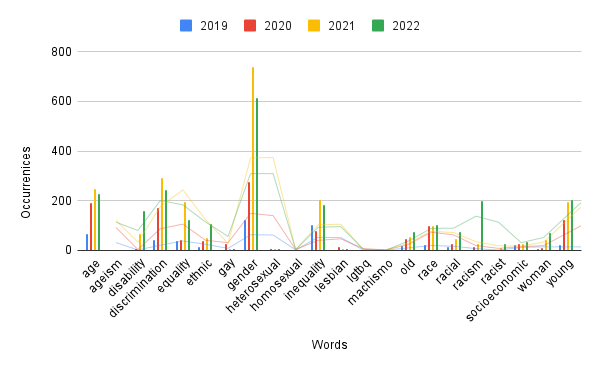
\includegraphics[width=\textwidth]{chart.png}
\centering
\caption{Number of word occurrences per year of study.} \label{chart}
\end{figure}
%%%%%%%%%%%%%%%%%%%%%%%%%%%%%%%%%%%%%%%%%%%%%%%%%%%%%%

\section{Discussion}
Based on the analysis results, it is evident that the primary focus of study is gender discrimination, accounting for over 75% of all the analyzed articles. The yearly increasing trend in the number of articles studying this phenomenon underscores the heightened awareness and concern that researchers have toward gender inequality. The slight drop in 2022 does not seem significant and does not undermine the overall growing trend\ref{tab2}.

The distribution of articles has increased across all types of discrimination over the years, with a particularly notable rise in racial discrimination studies. This surge could be tied to the influence of movements such as \#BlackLivesMatter \cite{nguyen2022black}, demonstrating the impact of social movements on academic interests and research trends.

Nevertheless, our analysis showed that some areas of discrimination, like sexual orientation, age, and disability, remain significantly under-represented in academic literature. This gap indicates potential areas for future research, with a need to broaden the understanding of discrimination experiences across various demographics within academia.

We also noted that institutional intervention plays a crucial role in addressing discrimination. However, the efficacy and impacts of such institutional efforts are not evenly distributed and require further investigation.

A promising outlook is emerging, nonetheless. The future landscape of academia seems to be moving toward more diversity and inclusion, which is evident in the decreased gender gap among post-doc students as reported in recent studies \cite{https://doi.org/10.1111/gwao.12549}. Although the changes are more apparent among younger generations, they are expected to permeate throughout the university and research institutes gradually.

While our study provides insights into the prevalence of various forms of discrimination in academic research, it is not without limitations. Our analysis is primarily dependent on the availability and accessibility of open-access articles, which means some relevant studies might have been missed. Moreover, the analysis relies on the presence of specific keywords in titles and abstracts, which may not fully capture the nuanced discussions within the full text of the articles. Future research should consider these limitations and strive for more comprehensive and nuanced methods for analyzing trends in academic research on discrimination.


\nocite{*}
\bibliographystyle{plainnat} % or any other style you like
\bibliography{refs}

\end{document}